\documentclass{article}
\usepackage{amsmath} % for \genfrac
\usepackage{tikz}
\usetikzlibrary{chains,positioning}

\tikzset{>=stealth} % nice arrow heads
%\tikzset{text depth=0pt}
\tikzstyle{box}=[rectangle,draw=blue,fill=white,text depth=0pt]
\tikzstyle{nobox}=[rectangle,fill=yellow,font=\itshape]
\tikzstyle{every node}=[on chain, join]
\tikzstyle{every join}=[->,shorten >=0.5pt,semithick]

% arguments to \genfrac: opening delimiter, closing del., width of line, style
% style: 0 \displaystyle, 1 \textstyle, 2 \scriptstyle, 3 \scriptscriptstyle
% long story short: to change the size, change the optional argument!
\newcommand{\twolines}[3][1]{$\genfrac{}{}{0pt}{#1}
{\text{\vphantom{Xg}#2}}{\text{\vphantom{Xg}#3}}$}

\begin{document}

\sffamily

\tikzset{node distance=2em}

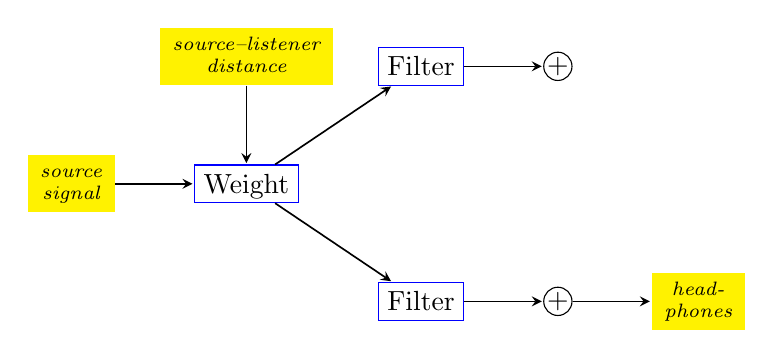
\begin{tikzpicture}[start chain]
\node[nobox] {\twolines{source}{signal}};
\node[box] (weight)  {Weight};
\begin{scope}[start chain=bla]
\node[nobox,above=of weight] {\twolines{source--listener}{distance}};
\chainin (weight);
\end{scope}
\begin{scope}[start branch=rbranch]
\node[box,on chain=going above right] (filterR) {Filter};
\node[circle,draw,inner sep=0pt] (plusR) {$+$};
\end{scope}
\node[box,on chain=going below right] (filterL) {Filter};
\node[circle,draw,inner sep=0pt] (plusL) {$+$};
\node[nobox] {\twolines{head-}{phones}};
\end{tikzpicture}

%\tikzstyle{every node}=[]

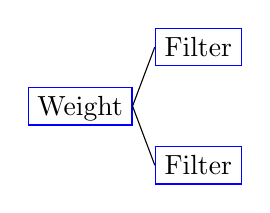
\begin{tikzpicture}
\begin{scope}[parent anchor=east,child anchor=west,grow=east,every node/.style=]
\node[box] (weight) {Weight}
child {node [box] (filterL) {Filter}}
child {node [box] (filterR) {Filter}};
\end{scope}

this text is not printed

\end{tikzpicture}

\tikzstyle{every node}=[]

\usetikzlibrary{decorations.pathmorphing}

\tikzstyle{every node}+=[rotate=rand*2,xshift=rand*.5ex,yshift=rand*.5ex]
\tikzstyle{every node}+=[xslant=rand*.03,yslant=rand*.03]
\tikzstyle{every node}+=[xscale=rand*.1+1,yscale=rand*.1+1]
\tikzstyle{every node}+=[decorate,decoration={random steps,segment length=10\pgflinewidth,amplitude=.5\pgflinewidth}]
\tikzstyle{every node}+=[decorate,decoration={bent,aspect=rnd*-.2}]

\usetikzlibrary{calc}

\tikzstyle{hvh}=[to path={
let \p{mid}=($(\tikztostart)!.5!(\tikztotarget)$) in
-- (\tikztostart -| \p{mid})
-- (\p{mid} |- \tikztotarget) \tikztonodes
-- (\tikztotarget)}]

\tikzstyle{vhv}=[to path={
let \p{mid}=($(\tikztostart)!.5!(\tikztotarget)$) in
-- (\tikztostart |- \p{mid})
-- (\p{mid} -| \tikztotarget) \tikztonodes
-- (\tikztotarget)}]

\begin{tikzpicture}
\node[box] (weight) {Weight};
\node[box,anchor=south west](filterL) at ($(weight.east)+(1cm, .5cm)$) {Filter};
\node[box,anchor=north west](filterR) at ($(weight.east)+(1cm,-.5cm)$) {Filter};
%\draw[->] (weight) to (filterL);
\path[->] (weight.east) edge[hvh] node[sloped,above,near end] {A} (filterL.west);
\draw (weight) to[vhv] node[auto=right] {B} (filterR);
\end{tikzpicture}

\begin{tikzpicture}
\path
node[box,double] (weight) {Weight}
(weight.east) % move to the right of weight and continue calculations from there
node[box,anchor=south west](filterL) at +(1cm, .5cm) {Filter}
node[box,anchor=north west](filterR) at +(1cm, -.5cm) {Filter};
\draw[->] (weight) -- (filterR);
\end{tikzpicture}

\usetikzlibrary{trees}

\begin{tikzpicture}[->]
\begin{scope}[growth parent anchor=east,parent anchor=east,child anchor=west,grow=east,sibling distance=2mm,level distance=2em,edge from parent fork right]
\node[box] (weight) {Weight}
child {node [box,anchor=north west] (filterR) {Filter right}}
child {node [box,anchor=south west] (filterL) {Filter left}};
\end{scope}
\end{tikzpicture}

\begin{tikzpicture}[->,child anchor=west,grow=east,sibling distance=2mm,level distance=2em,edge from parent path={(\tikzparentnode\tikzparentanchor) |- (\tikzchildnode\tikzchildanchor)}]
\node[box] (weight) {Weight}
node[circle,draw,fill,inner sep=0pt,minimum size=3\pgflinewidth] (fork) [right=of weight] {}
child {node [box,anchor=north west] (filterR) {Filter right}}
child {node [box,anchor=south west] (filterL) {Filter left}};
\path (weight) edge[-] (fork);
\end{tikzpicture}



\end{document}
